%----------------------- Thesis Master Document -----------------------------------%
%                                                                                  %
% Hacked together by Thomas Griffiths 2014-01-08 tmg994(at)uowmail.edu.au          %
% If you get stuck read my comments here and in the preamble (thesispreamble.tex). %
% Hopefully they can help you find your answers will be I highly reccomend making  %
% friends with Google and http://tex.stackexchange.com/, the truth is out there.   %
%                                                                                  %
%----------------------------------------------------------------------------------%

%------------------------ Preamble and bibliography resources
\documentclass[12pt,oneside]{book}
%--------------- UOW Thesis Preamble ----------------------------------------%
% Thomas Griffiths 2013-07-16 tmg994@uowmail.edu.au                          %
%                                                                            %
% I encourage you to read the documentation for each of the packages below,  %
% they contain instructions for implementation and examples of their use.    %
% If you get stuck read my comments, hopefully they can help you find where  %
% your answers will be. I highly reccomend making friends with señor Google, %
% he knows quite a bit. The wikibook on LaTeX is also very helpful:          %
% http://en.wikibooks.org/wiki/LaTeX/                                        %
% The packages I've loaded here are the bare basics. and mainly deal with    %
% formatting, captions and things. There are thousands of packages out there %
% for all the disciplines and formatting you might need. Google what you're  %
% looking for and the keywords 'LaTeX' and 'package', You'll probably find   %
% what you're looking for. I encourage you to look on ctan, www.ctan.org/‎,   %
% for packages that might be relevant to your degree. If you're in science I % 
% can recomend the siunitx and the chemmachro (or mhchem) package. They make %
% it really easy to typeset chemical equations, any quantity with units and  %
% scientific notation.                                                       %
%                                                                            %
%----------------------------------------------------------------------------%

\usepackage{geometry}
	\geometry{a4paper,inner=4cm, outer=2cm, top=3cm, bottom=2cm}
	% Dimensions from UOW thesis guidelines.
	\pdfpagewidth=\paperwidth 
	\pdfpageheight=\paperheight
	% This acts as a failsafe to ensure things aren't stretched or moved when it's finally printed as a PDF.

%\usepackage[parfill]{parskip} 
% Activate to begin paragraphs with an empty (return) line, comment out the indent below if you chose the return line option.

\setlength{\parindent}{4ex}	% Sets the length of the paragraph indent. Current setup has a an indent. Disable this if you activate the return line above.
	
\usepackage{setspace}
% Double or one and a half spacing.
	
\usepackage{graphicx}
	\DeclareGraphicsRule{.tif}{png}{.png}{`convert #1 `dirname #1`/`basename #1 .tif`.png}
% Graphics. Remove me and you won't have any figures, and that would be very boring.

\usepackage[usenames,dvipsnames,svgnames,table]{xcolor}
% Adds the ability to make coloured text and lines throughout the document. See documentation for xcolor.

%-------------------- Tables, figures and captions
\usepackage[font={small},labelfont={bf},margin=4ex]{caption}
% Makes bold labeled and smaller font captions. Must be loaded before the longtable package to avoid conflicts! 

\usepackage{longtable} 
% Long tables (more than one page). Different headers and footers for beginning and end pages, etc.

\usepackage{afterpage} 
% Make a longtable start on the next clear page, but fills the previous one with text first (no random gaps in the text-from long tables anymore! Man, the day I discovered this...)

\usepackage{booktabs} 
% Nice looking tables and lines in tables

\usepackage{multirow} 
% Entries in tables over multiple rows

\usepackage{lscape} 
% Pages in landscape

\usepackage{pdflscape} 
% Landscape pages also rotated in the pdf

\usepackage{wrapfig} 
% Allows figures that don't take up the entire width of the page, wrapping the text around the figure

%\usepackage[position=top,singlelinecheck=false,captionskip=4pt]{subfig} 
% Multiple figures in an individual figure. Fig. 1 a, b, c, etc. each with, or without, it's own individual caption, and with a global caption for all sub figures.

%-------------------- Special symbols and fonts
\usepackage{amssymb} 
% Maths symbols

%-------------------- Document sections, headers, footers, and bibliography
\usepackage{fancyhdr}											
% for creating different headers and footers

%-------------------- Bibliography
\usepackage[backend=biber,articletitle=true,style=chem-rsc,doi=false]{biblatex}
% This is the package that lets you create a bibliography. I recommend reading the biblatex documentation to understand all the options i've specified here. BibLaTeX was created to replace BibTeX. It has lots of extra fields and options. I'm also using the biber backend here rather than the default, it copes with unicode and so can deal with accented characters easily.

% Currently this is set up to use RSC style references with article titles displayed.

% Traditionally you would use BibTeX, a special build of TeX, the newer biblatex package is a more powerful bibliograpy management tool for LaTeX. You can make multiple chapter based bibliographies, footnote bibliographes, sort your references by date, author, order cited, essentially by any bit of citation data you happen to have. You can also have a seperate library with a differnet format for say books and articles. Or if you're a PhD student, the thesis references and your publications.

%\usepackage[numbers,super,comma,sort&compress]{natbib}				
	%\setcitestyle{square}										
	% places citations in square brackets to helps to distinguish between powers and citations
%This is the old natbib package that meshes with bibtex (rather than using the newer biblatex). It's here mainly for legacy purposes. Try to shift to biblatex if you can, it is cleaner in it's implementation and creating a custom citation style is easier then with bibtex.

\usepackage[unicode=true,colorlinks=true,linkcolor=black,citecolor=black,urlcolor=black,breaklinks=true]{hyperref}
% The hyperref package allows you to have clickable links in your pdf. It also allows you to have the mailto link associated with your name. It can be  a bit finicky, so load it last.

%-------------------- Command renewals, New commands etc.
\renewcommand{\thefootnote}{\alph{footnote}}							
%letters for footnotes instead of numbers to avoid confusion with references.
 % this must be left as \input, \include is giving me a hard time here and only here.
\usepackage[]{bradleythesistitlepage}
% Creates the title page in accordance with UOW guidelines, includes the definition of the extra fields in \maketitle
\addbibresource{your_bibliography.bib}

%------------------------ Main Document --------------------------
\begin{document}
    \onehalfspace
	
%-------------- Information For The Title Page
% Title page info (see uowthesistitlepage package)
    \title{Distributed Vision-Based Target Tracking Control Using Multiple Mobile Robots} 
    \author{Anthony Le and Ryan Clue}
    % Full name, and any degrees held.
    
    \date{May 5, 2017} 
    % Month Year, alternatively use the \today macro for Month dd, yyyy.
    
    \degree{Bachelor of Sciences } 
    % Write it in full: e.g. Bachelor of Science Medicinal Chemistry Honours
    
    \supervisor[2]{Dr. Jing Wang \& Dr. In Soo Ahn} 
    % The optional argument (default 1) in square brackets is the number of supervisors. In the Curly braces list your supervisor(s) seperated by commas.
    
    %\cosupervisor[1]{Dr. C. O. Supervisor}
    % The same as the supervisor command above. This command is optional.
    
   % \school{Bradley University} 
    % e.g Chemistry

%-------------- Front Matter
    \frontmatter
    \maketitle
    
    %\declaration
    
    % These \phantomsection are to ensure that the hyperref package hyperlinks to the correct page in the electronic pdf. If you turn hyperref off they don't do anything so they can just stay here.
\phantomsection\addcontentsline{toc}{chapter}{Abstract}
\chapter*{Abstract} % Starred chapter=chapter with no number.

In this project, a distributed vision-based control system is designed for multiple mobile robots to address the target tracking problem while maintaining the specified formation among robots. The system mainly consists of two modules. One is for target identification and the other is for target tracking control. In the target identification module, the robot is controlled to pivot around its center and perform a survey of the environment using its on-board vision sensor. In the target tracking control module, a leader-follower control strategy is adopted to solve the target tracking and formation control problem of multiple robots. The proposed distributed vision-based control is experimentally tested using three QBot2s from Quanser, Inc. 
    \chapter*{Acknowledgments}

%-------------- Table of contents
    \cleardoublepage
    \phantomsection \pdfbookmark[0]{Contents}{Contents} 
    \tableofcontents
    
    \listoffigures
    % These \phantomsection are to ensure that the hyperref package hyperlinks to the correct page in the electronic pdf. If you turn hyperref off they don't do anything so they can just stay here.

%-------------- Chapters
    \cleardoublepage
    \mainmatter
    \chapter{Introduction}


\section{Motivation}
Distributed control of multiple unmanned autonomous robots (UARs) has been the subject of intensive research in recent years due to the potential applications in search and rescue missions, surveillance and reconnaissance, environmental sensing and monitoring, intelligent transportation and threat isolation/evasion, and obstacle evasion [1]. There are many practical commercial, civil and military applications that may benefit from advancements in UAR control strategies and algorithms from this area of research. 

\section{Related work}
Methods for successfully coordinating multiple robots to autonomously encircle a target point have been put forth by several research papers.  These distributed controls assume communication the robots to communicate their kinematic state variables between one another, and consequently researchers have designed their algorithms in ways that minimize the number of communication channels required between robots.  However, there has not been nearly as much research done that attempt to implement coordinated encirclement that rely entirely on each individual robot’s vision sensors.

A review of prior work at Bradley and research literature was conducted by our team during the conception phase of the project.  This included a review of e prior Class of 2016 Senior Project, Cooperative Control of Heterogeneous Mobile Robots Network [cite ref 1?]. The 2016 research and capstone project experience using the QBot2 robots was leveraged in our project. The 2016 project tested cooperative control using the QBot2 platform including the Qbot2 Camera and the Kinect RGBD camera for localization.  Wifi communication was used to exchange position information among robots. Consensus and formation stabilization problems were studied. 

Our project also researched and references another work, highly relevant to our 2017 project objectives. Decentralized multi-robot encirclement of a 3D target with guaranteed collision avoidance for object tracking and encirclement by Franchi, Stegagno, and Oriolo, [cite ref 2]. Their work on 3-D (and 2-D) and distributed collaborative control is extensive and leverages research going back to 2001.   Their findings delivers a control framework for achieving encirclement of a target moving in a 3D space using multiple robots, image-only sensing, and requiring local communication between exactly two other members of the encircling group of robots. 

An additional consideration, for a vision-only sensing strategy was image processing techniques and algorithms.  We relied on Peter Corke’s book “Robotics, Vision and Control” as well as his Matlab toolbox for much of our image processing.  The academic tutorials packaged with the Qbot2 were also valuable resources.  It is worth mentioning that systems in the literature utilizing visual-only sensing generally assumed 360-degree robot sensing (e.g. fisheye camera). Ref 1 Research (extracts below) utilized a 240deg field of view sensor and a laser range finder for identification and locating targets to support inputs to their control strategies.  Because the Qbot2 cameras have less than a 90-degree field-of-view, our design would have to incorporate additional logic to locate targets outside the robot’s visual range.

    \chapter{Problem Formulation}


\section{Kinematic Model of Mobile Robots}

Depending on whether the robot is following a target or leader robots, two separate control modules are used. Both modules use a Cartesian coordinate system and follow a target point, which is obtained by transforming the current or previous result of the image processing module with respect to the robot’s current position.

\section{Vision-based control}
The purpose of the vision-based control is to provide a target point to the kinematic control, which it accomplishes by processing the Qbot2’s color images and depth images. This control should also provide additional information as to whether the target point it provides should be considered valid or not.


\section{Project Objectives, Goals, and Approach}
The goal of our project is to design distributed vision-based control algorithms for mobile robots and to implement and validate the proposed algorithms. The primary project tasks (research, concept definition, design, and demonstration) tasks included:

\begin{itemize}
\item	Design a target identification (detect and locate) module based on RGB image features obtained from a vision sensor
\item	Design a target tracking algorithm based on robot model linearization
\item	Design a leader-follower formation control algorithm based on depth and image features provided from the target identification module 
\item	Design a state machine to coordinate target identification module and target control module and communications between Robots
\item	Integrate and validate the proposed distributed controls through experimentation in a controlled lab environment
\end{itemize}


\section{Project Assumptions}
The Lab environment, limitations of the research and practical limitations (and availability) of fully operational equipment are also considered.  

\begin{itemize}
\item	The lab environment will be a well-lit, indoor area
\item	The target will remain on the same level plane as the robots (2D motion tracking).  
\item	The target will not move faster than the Qbot2s maximum velocity (0.7 m/s).  
\item	The target will be a solid colored, basketball-sized sphere.  
\item	The environment will be reasonably free of similarly colored objects.  
\item	As stated above the multiple robots must use same control strategy.

\end{itemize}

    \chapter{Design of Distributed Vision-based Control}


\section{Design approach}

The basic “system” is comprised of the QBot2 Mobile Robot and QUARK Control Software on a host computer.  The full “system” is comprised of multiple QBot2s collaboratively tracking a single target with the Quark Control Software Computer.  Note: An assumption is that the Quark Control Software on the host computer could be ported entirely to the robots, given sufficient processing and communications, to attain higher autonomy and actual decentralization of the system.  The target in the experiment is a round ball that is detected, located, and tracked by the multiple QBot2s.    
Subsystems for the basic system, a single QBot2, include: the Qbot2 mechanical/motors/control subsystem, the sensing/image processing subsystem, and the communications/processing subsystems (on the Qbot2 and the Host computer). 

\section{QBot2 Mobile Robot and QUARC Platform}

The QBot2 utilizes QUARC’s HIL software suite to allow users to design their program using Matlab and Simulink.  The Simulink model and Matlab code are translated to C++ code by the QUARC software and compiled automatically on the Qbot2’s computer.

\subsection{Hardware}

The QBot2 comes equipped with a differential drive robot base which has a maximum speed of 0.7m/s. A v1 Kinect-for-Xbox mounted on the robot base provides both color and distance vision information.  The RGB image that has a default resolution of 640 × 480 pixels and a 57° × 43° field of view.  The depth image has a resolution of 640 × 480 pixels, approximately 52.5° × 41° field of view, and measures distances from 0.5m to 6.0m. It is worth noting that the accuracy of the depth map depends on the detail of the grid projected by the IR emitter, the actual accuracy of the depth image is significantly lower than a resolution of 640x480 implies.   QBots use IEEE 802.11 b/g/n protocol for communication between the computer and QBot2. TCP/IP protocol is utilized, with each QBot2 using a statically assigned IP address. More information on sensors can be found in the appendix.

\begin{figure}[htbp] %  figure placement: here, top, bottom, or page
     \centering
     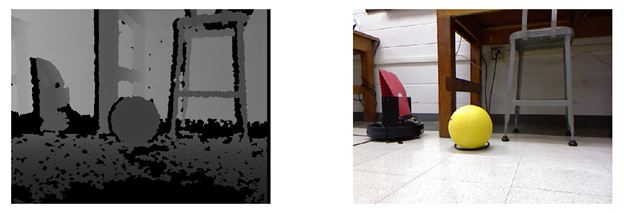
\includegraphics[width=5in]{1.png} 
     \caption{Side-By-Side of Color and Depth Images}
     \label{fig:1}
  \end{figure}     


\begin{figure}[htbp] %  figure placement: here, top, bottom, or page
     \centering
     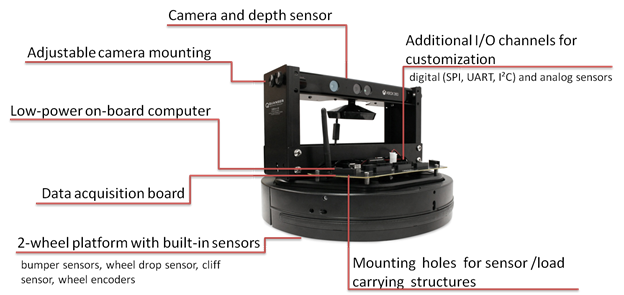
\includegraphics[width=4in]{2.png} 
     \caption{QBot2 Mobile Robot}
     \label{fig:2}
  \end{figure}     


\subsection{Software}
To connect to the QBOT2 A host-target real-time control system [2] is utilized.   As shown in Figure 3-2, the target QBOT2 computer is connected wirelessly with the host computer on which the SIMULINK model is running. The control algorithms are developed in MATLAB/SIMULINK with QUARC on the host computer. The control models are cross-compiled and downloaded to the target computer in real time. 


\begin{figure}[htbp]
\begin{center}
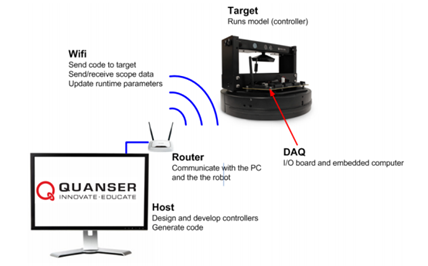
\includegraphics[width=5in]{3}
\caption{Host Computer / Wi-Fi Router to Qbot Communications Connectivity} \label{fig:3}
\end{center}
\end{figure}

\section{Target Identification}
\subsection{Interface and inputs to Target Control}
The result of the vision control system is a target location given in 2D Cartesian coordinates. The origin of this coordinate plane is at the Qbot2’s camera position, the positive X axis extends in same the direction the Kinect is facing and the positive Y axis extends to the left (or “port” side) of the Kinect.  The motion control module will then transform this point according to its current kinematic state.   This is target point is the basic interface between the target identification module and the motion control.

Based on the 2016 Senior Project, and research of alternatives, we chose to use the color image for object/target recognition and the depth image for determining distance to the target. Our choice was driven primarily by practical QBot2 processing limitations and timing restrictions prohibiting potentially more robust methods of object detection (see Appendix).

\subsection{Acquire Y Component of Target Location from Color Imagel}
We perform all object recognition on the color image.  Consequently, color image processing is the primary bottleneck in system performance.  We initially selected color thresholding with blob detection because it is the easiest image processing method to implement.  Although we did pursue alternative methods of image processing, these implementations were unable to meet our performance requirements due to limitations of the Qbot2 hardware.  Therefore, color thresholding with blob detection was selected because it had a significantly lower performance requirement while also producing adequate results. 

The first stage of image processing, color thresholding, highlights all elements of the image that correspond to our target’s color.  During this stage, pixels with RGB values that fall within a pre-determined range are replaced by ‘1’ in the binary output image, while all other values are replaced by ‘0’.  

Blob detection is applied to the binary output image from color thresholding.  The goal is to identify the largest grouping of neighboring, non-zero values.  Then, for each group (or “blob”) of neighboring pixels, we calculate its centroid by finding the mean index of all pixels contained in that blob.  This means that the accuracy of the blob corresponding to our target object is unaffected by “noise” from similar colors appearing elsewhere in the image.  It should be noted that the accuracy of this method is therefore entirely dependent on the color thresholding result.  

\begin{figure}[htbp]
\begin{center}
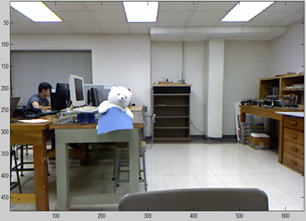
\includegraphics[width=5in]{4}
\caption{Before Processing - Color Thresholding and Blob Detection} \label{fig:4}
\end{center}
\end{figure}

\begin{figure}[htbp]
\begin{center}
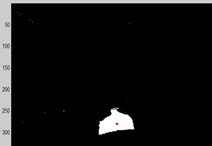
\includegraphics[width=5in]{5}
\caption{After Processing - Color Thresholding and Blob Detection} \label{fig:5}
\end{center}
\end{figure}
The blob detection outputs a list of centroids and corresponding blob sizes.  If the blob size of the largest blob is greater than some pre-determined threshold value, our system will use that centroid for the target’s coordinates on the RGB image plane. 


\subsection{Acquire X Component of Target Location from Depth Image}
The target’s location on the depth map can be estimated by translating points from the color image plane to the depth image plane.  We calculated this using the ratio between the two images’ field-of-view and the estimated angle from the RGB image.

\begin{figure}[htbp]
\begin{center}
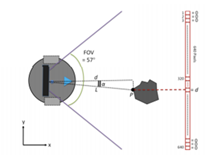
\includegraphics[width=5in]{6}
\caption{Target Localization} \label{fig:6}
\end{center}
\end{figure}

\begin{equation}
∝_T=(L_{color}/2-X_{color} )(¬(FOV_{color}-x)/L_{color} )
\end{equation}

\begin{figure}[htbp]
\begin{center}
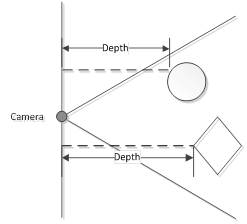
\includegraphics[width=5in]{7}
\caption{Host Computer / Wi-Fi Router to Qbot Communications Connectivity} \label{fig:7}
\end{center}
\end{figure}

\begin{equation}
〖XY〗_{depth}=(〖FOV〗_{color}/L_{color} )(L_{depth}/〖FOV〗_{depth} ) 〖∙XY〗_{color}+offset
\end{equation}
\begin{equation}
X_T=〖Image〗_{depth} (X_{depth},Y_{depth})
\end{equation}
\begin{equation}
Y_T=X_T∙tan⁡(∝_T)
\end{equation}
\section{Motion Control}
\subsection{Encirclement}
The target control module relies on received target coordinates from the image processing module and the robot’s  x,y, and theta. These are inputs which allow for formulation of encirclement.  From the robot’s x,y, and theta values, we transform these values to the appropriate kinematic model for the QBot2. From this kinematic model, we transform the cartesian local coordinate system to a cylindrical coordinate system. The length between the two wheels of the QBot is 0.0235 meters. To find the forward point location of the robot, we use,
\begin{equation}
	P_x=x+0.0235*cos⁡(θ)
\end{equation}
\begin{equation}
	P_y=y+0.0235*sin⁡(θ)
\end{equation}

Following, we want to define qi,
\begin{equation}
	q_i=〖(ρ〗_i  ϕ_i)
\end{equation}
	
and convert these values by,
\begin{equation}
	ρ(p)=√((p_x^2+p_y^2 ) )
\end{equation}
	
\begin{equation}
	ϕ(p)=〖atan〗^2⁡〖〖(P〗_y,Px) 〗
\end{equation}
	

where p is the pose of the model.

ρ ̇ and ϕ ̇ are the forward velocity and angular velocity computed by:
----
\begin{equation}
	ρ ̇=k_r*(ρ_s- ρ_d)	(6)
\end{equation}
		
\begin{equation}
	ϕ ̇=ω_d
\end{equation}
	

where $k_r$  is the porportional gain and $ρ_s$ is the size of the encirclement radius. $ρ_d$ is the approximate distance from the robot to the target given from the inverse kinematics and image processing modules.

We then use the Jacobian matrix of the difference between the target and robot where Px and Py is the X and Y coordinates of the robot and Pxt and Pyt is the X and Y coordinates of the target in relation to the robot’s coordinate frame. The difference of the robots X and Y locations can be reduced to Pxd and Pyd. and the following Jacobian  matrix can be computed
\begin{equation}
		J_i=((P_xd/√(P_xd^2+P_yd^2 )  P_yd/√(P_xd^2+P_yd^2 )  〖-P〗_yd/(P_xd^2+P_yd^2 )P_xd/(P_xd^2+P_yd^2 )))   
\end{equation}


	


From the Jacobian, the following input velocities Ux and Uy can be computed
\begin{equation}
		[U_x,U_y ]=J_i^(-1)*[ρ ̇,ϕ ̇]
\end{equation}
	
For the velocity inputs, $U_x$ and $U_y$ , they are transformed using the inverse kinematic equations
\begin{equation}
			p^(-1)=((cos⁡(θ)-0.0235*sin⁡(θ)@sin⁡(θ)0.0235*cos⁡(θ) ))^(-1)
\end{equation}
	

to find $V_c$ and $ω_c$,
\begin{equation}
[V_c,ω_c ]=p^(-1)*[U_x,U_y]
\end{equation}	

Once $V_c$ and $W_c$ are found, using
\begin{equation}
V_r=V_c+1/2* .0235*2*W_c
\end{equation}
\begin{equation}
	V_L=V_c-1/2* .0235*2*W_c
\end{equation}
	

	
we can find velocities of the right and left wheels, Vr and VL.

Right and left wheel velocities are then sent to the HIL Write block which sends data to the 2000 and 2001 ports of the QBot2 for the left and right wheels, respectively.
The QBot2 stores wheel encoder data to allow calculation of actual right and left wheel velocities. This data is taken from the HIL Read block. For each wheel encoder ticks, we can determine the velocity of each wheel. The robot’s x,y, and θ values are then updated and sent back into the control module using Vc and θ where,
\begin{equation}
V_c=0.5*(V_L+V_r)
\end{equation}
\begin{equation}
Θ=1/0.235*(V_r-V_L)
\end{equation}
	

	


From $V_c$ and $ω_c$, we can determine the robot’s X, Y, and θ values by calculating the integrals for
\begin{equation}
x ̇=cos⁡(θ)*V_c
\end{equation}
\begin{equation}
y ̇=sin⁡(θ)*V_c
\end{equation}
\begin{equation}
	θ̇=ω	
\end{equation}

	

		

\subsection{Encirclement}
Leader-follower control module is used for distributed multi-robot coordination. The leader-follower control module does not take into account inverse kinematics. And, the image processing is used to localize the leader robot coordinates ($𝑥_𝑟$  , $𝑦_𝑟$) in the vision sensor range. Given the radial distance of the target, $V_c$ and $ω_c$ are calculated. A follow distance of 0.5 meters and gains  Kw = 0.5 and Kv = 0.2 were defined as per limitations for the QBot.
To determine $V_c$ and $ω_c$,
\begin{equation}
	V_c=K_v*√(x_t^2+y_t^2 )-0.5	(15)
\end{equation}

\begin{equation}
	ω_c=-K_w*arctan⁡(x_t,y_t)
\end{equation}


where xt and yt are the positions of the target in relation to the robot’s local coordinate frame.
One should note the limits for angular and forward velocity are set to .2 m/s.



\section{Event-based System Control}
\subsection{Implementation}
The Simulink model is configured using the HIL block from the QUARC toolbox.  This enables users to more easily run their simulations in a virtual environment as well as on actual hardware.  The project must also be configured to communicate with a specific IP address, which can be done through the QUARC add-on options menu in Simulink.  It is also important to set the sample time configure the “Solver” pane of the Simulink model configuration.  It is important to select the “ode1” and “fixed-step” options.  Additionally, when performing operations on images or large arrays of data, it is recommended that users select a sample frequency no greater than 15Hz.  Our experiments used a 10Hz sample frequency.
\subsection{Tasks Coordination}
Our system would need to switch between two modes of operation depending on whether or not the target was in view.   Stateflow was used to control the varying states in our model. Models for both target encirclement and leader-follower used similar simulink and stateflow models with differences only in controls and how often a search was made. In both models, search mode is done by toggling between image processing and rotating. Once the desired accuracy is obtained from blob detection, the state switched to the control module.  The target encirclement model only searches for target every set time-interaction whereas leader-follower will search for a target every other time-step.

\begin{figure}[htbp]
\begin{center}
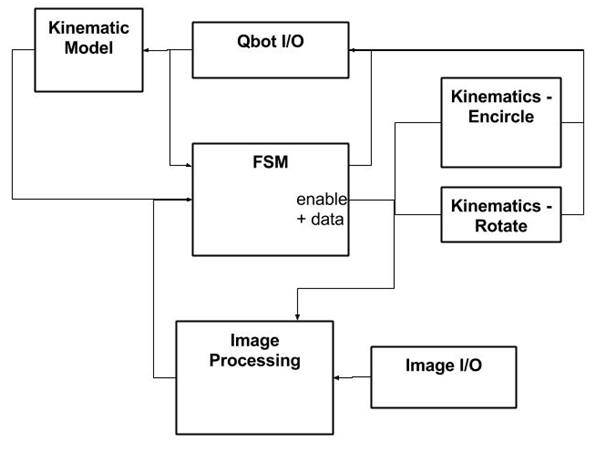
\includegraphics[width=5in]{8}
\caption{Abstracted View of Simulink Diagram} \label{fig:8}
\end{center}
\end{figure}

\subsection{Target Encirclement - Finite State Machine}
In the stateflow for target encirclement control, various enable switches allow triggering of different modules. The system starts off with all enable switches off. While entering target acquisition mode, image processing module is enabled and determines if an image centroid can be made. If no centroid is found, the QBot2 will rotate 15 degrees on its axis and wait for the cameras to update. If a centroid can be made, it checks whether the pixel size of the image is greater than a certain value. In our case, a yellow ball or box is used. If 30 pixels are connected, the robot will continue into the encirclement module. Data from the image processing, such as the robot’s x, y, and theta, is also sent to the encirclement module. From this module, the target location is stored and encirclement is based on this value. After 120 seconds, the encirclement ceases and target acquisition mode begins again

\begin{figure}[htbp]
\begin{center}
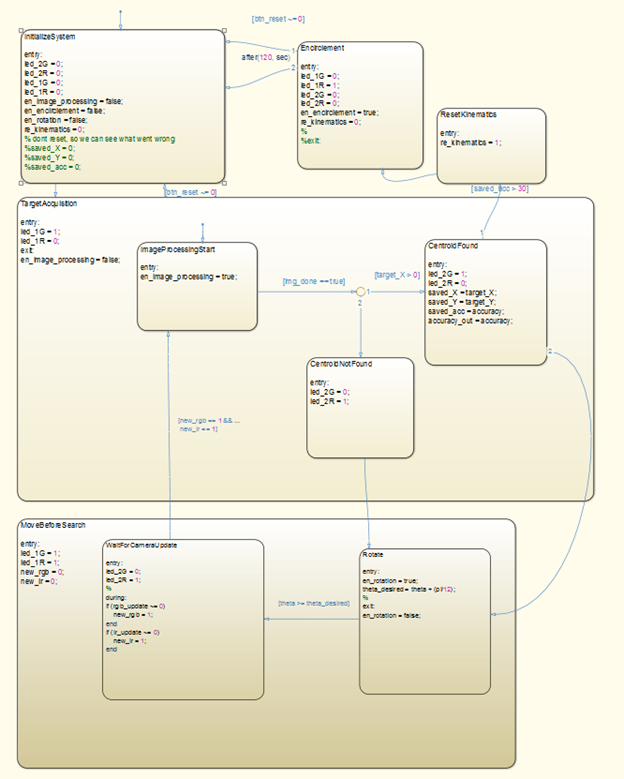
\includegraphics[width=5in]{9}
\caption{Event-based System Control: Encirclement Control} \label{fig:9}
\end{center}
\end{figure}

\subsection{Leader-Follower - Finite State Machine}

Leader-follower control is similar to target encirclement control. However, instead of returning to Target Acquisition mode, the target will continue to follow any centroid even if the pixel count is less than 30. The process is done by continually switching from image processing and the leader-follower control module. If no centroid is found, the target will return into Target Acquisition mode.


\begin{figure}[htbp] 
\begin{center}
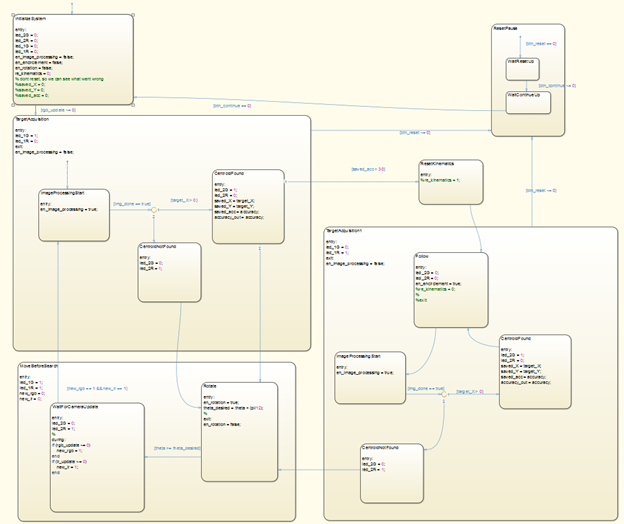
\includegraphics[width=5in]{10}
\caption{Event-based System Control:Ledaer-Follower Control} \label{fig:10}
\end{center}
\end{figure}


\section{Experiments}
A curriculum for the QBot was provided to allow interfacing and familiarity of the QBot2 and its software package, QUARC. The curriculum covers topics ranging from QBot communication, integration, kinematics and vision guided control. Advanced topics such as path planning, mapping, and localization are also covered. Each section provides an in-depth tutorial for the understanding of the QBot’s capabilities. Tutorials for blob detection, line-following, and kinematics were most referenced in our project.
Various simulations for the control module were implemented in Matlab and Simulink. These demonstrations assumed constant communication between robots. For encirclement control, single robot to a multiple robot models were simulated to show proof of concept. Refer to the appendix for more information.
From simulation, the first series of experiments were conducted. Using a predefined target point, encirclement of a single robot was tested. Our next iteration, using blob detection, allowed us to capture and encircle the target point. The next iteration consisted of determining which method of control was needed to allow coordination between robots. Stateflow was used to control different modules efficiently. Following, a leader-follower model was implemented for successive robots.

\section{Results}
Experimental results can be seen in figures below. Target encirclement was achieved by the target robot. Using the appropriate thresholds for the color yellow, the robot was able to identify the target.
\begin{figure}[htbp]
\begin{center}
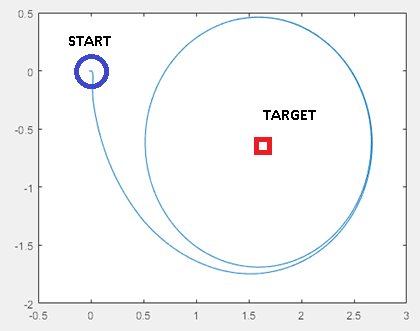
\includegraphics[width=5in]{11}
\caption{Phase Plot of Encirclement Robot} \label{fig:11}
\end{center}
\end{figure}

\begin{figure}[htbp]
\begin{center}
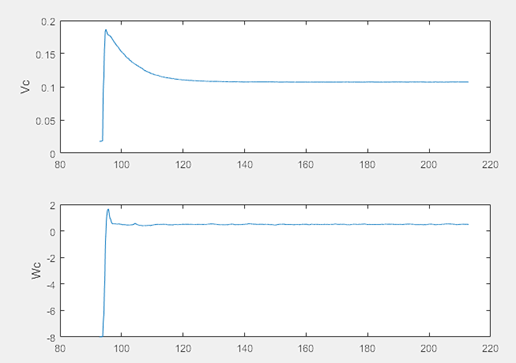
\includegraphics[width=5in]{12}
\caption{Forward and Angular Velocities of Encirclement Robot} \label{fig:12}
\end{center}
\end{figure}

\begin{figure}[htbp]
\begin{center}
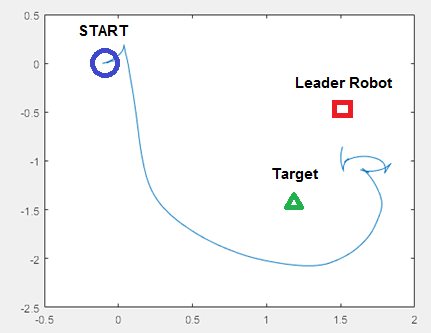
\includegraphics[width=5in]{13}
\caption{Phase Plot of Leader-Follower Robot} \label{fig:13}
\end{center}
\end{figure}

\begin{figure}[htbp]
\begin{center}
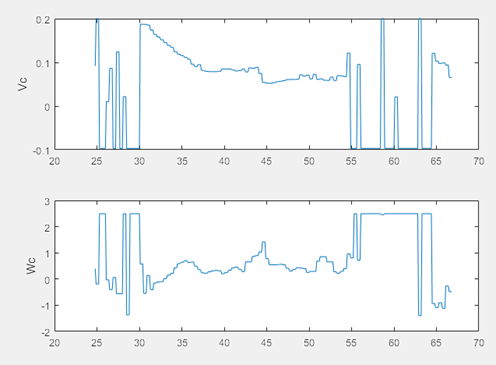
\includegraphics[width=5in]{14}
\caption{Forward and Angular Velocities of Leader-Follower Robot} \label{fig:14}
\end{center}
\end{figure}

Encirclement control can be seen in the following: https://www.youtube.com/watch?v=VHpTNNhiLG4
Leader-follower control can be seen in the following: https://www.youtube.com/watch?v=bO5DHXQCITw



    \chapter{Project Management}


\section{Division of Labor}
Ryan Clue implemented our image processing methods, created the initial Stateflow model, and provided the Simulink design for integrating the image processing modules with the kinematic modules.

Anthony Le implemented our kinematic control systems, created our Matlab data logging module, and extended our Stateflow model for the Leader-Follower program.

Anthony and Ryan worked jointly to debug and troubleshoot.
    \chapter{Discussion}

\section{Impact of the Design}
Our design allows limited communication and sensing among all robots. Assuming a leader and its peripheral robots, we can obtain encirclement with each consecutive robot containing a smaller and smaller encirclement radii. This two part modular design allows for classifying the leader and followers and allows for increased modularity and customization if needed. With Stateflow, replacing a certain image processing or control module is as simple as replacing or rewriting a Simulink block. Creating simulations for certain environments can also be implemented using Stateflow.
The overall design can be implemented in search and rescue missions, environmental surveying, and much more.

\section{Future Work}
There are two areas that can be significantly improved or developed.

The first improvement would be to implement collision avoidance.  This would involve additional image processing as well as control logic.  The kinematic control can be improved to accommodate obstacle avoidance by scaling the encirclement radius as the Qbot2 approaches the obstacle in its path (ref encirclement paper).  As for identifying the obstacle, we believe that this can be accomplished identifying expected distance from the floor and identifying all image elements that deviate from that expected floor distance.  

The method of object recognition could also be improved. One possibility is using edge detection and performing a Hough Transform for the expected target object shape.
    \chapter{Conclusion}

Our project have demonstrated distributed vision-based target tracking control using mobile robots. We have achieved the project goals mentioned in Section 2.3 – that is to design a target identification (detect and locate) module based on RGB image features obtained from a vision sensor, to design a target tracking algorithm based on robot model linearization, to design a leader-follower formation control algorithm based on depth and image features provided from the target identification module, to design a state machine to coordinate target identification module and target control module and communications between robots, and to integrate and validate the proposed distributed controls through experimentation in a controlled lab environment. 
All the while, there were still problems with the upcoming design. The QBot2 does not contain enough processing power for the image processing that we desired – therefore, blob detection was used. A better target recognition algorithm, such as hough transforms, allows a more robust target detection method. Failures, such as the target being misclassified or kinematic issues, were also noted and fixed during implementation. The Qbot occasionally would reset and move backwards once a target object was found. We believe this may be an issue with misclassification or a faulty kinematic model. Another problem with the QBot concerned the updating of RGB and IR images. The middleware for the Simulink design block that increased a tick for every image update occasionally would not change. This prevented us from keeping track each time image processing was finished and delayed search mode.
Overall, this project demonstrated that minimized local communication and formation between robots is feasible. Future work, such as obstacle avoidance and improved image processing, can still be researched.
    
    
%-------------- Bibliography
    \cleardoublepage
    \phantomsection	\addcontentsline{toc}{chapter}{Bibliography}										
%    \printbibliography
    
    
\begin{thebibliography}{99}
\bibitem{}{“Cooperative Control of Heterogenous Mobile Robots Network.” [Online]. Available: http://ee.bradley.edu/projects/proj2016/mrn/. [Accessed:  14-Dec-2016].}

\bibitem{}{G. Bock, R. Hendrickson, J. Lamkin, B. Dhall, J. Wang, and I. S. Ahn, “Experiments of distributed control for multiple mobile robots with limited sensing/communication capacity,” in 2016 IEEE International Conference on Electro Information Technology (EIT), 2016, pp. 0559–0564.}
\bibitem{Oriolo}{G. Oriolo. Wmr control via dynamic feedback linearization: design, implementation and
experimental validation. {\it IEEE Trans. on Control Systems Technology}, 10:835–852, 2002.}
\bibitem{Oriolo}{Franchi, Stegagno, and Oriolo. Decentralized multi-robot encirclement of a 3D target with guaranteed collision avoidance. 2016}
\bibitem{Oriolo}{Freda and Oriolo. Vision-based interception of a moving target with a nonholonomic mobile robot. 2007}
\bibitem{Oriolo}{S. Miah, Lab 2: Trajectory Tracking Using Differential Drive Mobile Robots. 2016 .}
\bibitem{}{Cap 02.pdf. [Online]. Available: http://mayerle.deps.prof.ufsc.br/private/eps6405/Cap 2002.pdf. [Accessed: 14-Nov-2016]}
\bibitem{}{“Kinect for Windows Sensor Components and Specifications.” [Online]. Available: https://msdn.microsoft.com/en-us/library/jj131033.aspx. [Accessed: 14-Dec-2016].}

\bibitem{}{MRNProposalDocument.pdf. [Online]. Available: http://ee.bradley.edu/projects/proj2016/mrn/MRNProposalDocument.pdf.  [Accessed: 14-Nov-2016]}
\bibitem{}P. Corke, Robotics, Vision and Control - Fundamental Algorithms in MATLAB . Sep 2011
\bibitem{}{Quanser - QBot 2 for QUARC. [Online]. Available: http://www.quanser.com/products/qbot2. [Accessed: 14-Nov-2016].}

\end{thebibliography}

    

%-------------- Appendicies
    \cleardoublepage
    \appendix
    \chapter{Appendix One}
\section{The title of the first section}
The appendices work exactly the same way as chapters, they are numbered with letters rather than numbers though.
    \chapter{Appendix Two}
\section{The title of the first section}
    
\end{document}  

%---------------------------Notes-------------------------------
% Examples:

% Figure or Scheme (caption after)

% \begin{figure}
% \centering
% \input{figures/name_of_figure.tex}
% \caption[Short caption for table of figures]{Long caption for text body}
% \end{figure}

% Table (caption before)

% \begin{table}
% \centering
% \caption[Short caption for table of tables]{Long caption for text body}
% \input{figures/name_of_figure.tex}
% \end{table}

%-------------- 
% A list of Figures, put after the table of contents and uncomment to activate.
% \cleardoublepage
% \phantomsection \label{listoffigures}\addcontentsline{toc}{chapter}{List of Figures}
% \listoffigures

% A list of Schemes, put after the table of contents and uncomment to activate.
% \cleardoublepage
% \phantomsection \label{lisrofschemes}\addcontentsline{toc}{chapter}{List of Schemes} 
% \listofschemes

% A list of Tables, put after the table of contents and uncomment to activate.						
% \cleardoublepage
% \phantomsection \label{listoftables}\addcontentsline{toc}{chapter}{List of Tables} 
% \listoftables

%--------------
% Floats and centreing for tables can be a bit confusing if you have a seperate file for your tables. \begin{table}, \centering and \caption[]{} goes in the body text, *then* include the file closing with \end{table to ensure correct float placement. If you put the float and centering in the included file along with the body of the table you're going to have a bad time. Of courese, this is only if you are calling in your tables as seperate files, not leaving them in the text. Also note the american spelling of center (not the standard AU centre).

%-------------- 
% The difference between \input and \include is thus: \include creates an aux file for the included file, \input does not. \include is good for large files, like a chapter, since LaTeX won't reread the file if no changes have been made. \input is better for small inputs like data tables, since it doesn't create an aux file for the inputted file, it is read each and every time LaTeX is run. Additionally you *CAN* nest \input commands. you *CANNOT* nest \include commands.
